\documentclass[11pt,final]{article}
\usepackage{a4wide}
\usepackage{graphicx}              % figures
\usepackage{listings}              % source code
\usepackage{hyperref}              % navigation
\usepackage{booktabs}
\usepackage[small]{caption}
\usepackage{color}
\usepackage{xspace}
\usepackage{mathptmx}
\setcounter{tocdepth}{1}

\parindent0mm                      % this looks better in short paragraphs
\definecolor{lightgray}{rgb}{.95,.95,.95}
\definecolor{middlegray}{rgb}{.55,.55,.55}
\lstset{
  basicstyle=\footnotesize\ttfamily,
  keywordstyle=\bfseries\ttfamily,
  commentstyle=\color{middlegray}\ttfamily,
  tabsize=2,
  numbers=none,
  numberstyle=\tiny,
  numberblanklines=false,
  stepnumber=1,
  numbersep=10pt,
  language=C,
  xleftmargin=0pt,
  backgroundcolor=\color{lightgray}
}

\newcommand{\classname}[1]{\emph{#1}}
\newcommand{\keyword}[1]{\lstinline{#1}}
\newcommand{\Gt}[0]{\emph{GenomeTools}\xspace}

\title{The \Gt Developer's Guide}
\author{Sascha Steinbiss, Gordon Gremme and Stefan
        Kurtz\thanks{please send comments to:
        \texttt{steinbiss@zbh.uni-hamburg.de}}}


\begin{document}
\maketitle
\tableofcontents


\section{Introduction}
This document describes design properties and coding guidelines for the \Gt
genome analysis system. The goal of the \Gt environment is to provide a
well understandable, comprehensive and most importantly reusable set of classes
and modules to aid in the development of C-based bioinformatics applications.

The expected gain in productivity is only possible to achieve if all
components of the \Gt behave in a similar way -- or so to say -- in a way which
is least surprising to the user (which is, in this case, a programmer).
Thus we ask all developers contributing code to the \Gt to adhere to a common
set of rules which make it easier for others to reuse the products of
everyone's hard work.


\section{Object-oriented design}
\subsection{Classes}

The central component type in \Gt is the \emph{class}. Structuring the C code
into classes and modules gives us a unified design approach which simplifies
thinking about design issues and avoids the code base becoming monolithic, a
problem often encountered in C programs.

\subsubsection{Simple classes}

For most classes, a simple class suffices. A simple class is a class which does
not inherit from other classes and from which no other classes inherit. Using
mostly simple classes avoids the problems of large class hierarchies, namely
the interdependence of classes which inherit from one another. The major
advantage of simple classes over simple C structs is information hiding.

\subsubsection{Implementing simple classes}
\label {simpleclasses}

We describe now how to implement a simple class using the string class
\keyword{str.[ch]} of \Gt as an example. The interface to a class is always
given in the \keyword{.h} header file (\keyword{str.h} in our example). To
achieve information hiding the header file cannot contain implementation details
of the class. The implementation can always be found in the corresponding
\keyword{.c} file (\keyword{str.c} in our example). Therefore, we start with
the following C construct to define our \keyword{GtStr} class in
\keyword{str.h}:

\begin{lstlisting}
typedef struct GtStr GtStr;
\end{lstlisting}

This seldomly used feature of C introduces a new data type named
\classname{GtStr} which is a synonym for the \keyword{struct GtStr} data type,
which needs not to be known at this point. In the scope of the header file, the
new data type \keyword{GtStr} cannot be used, since its size is unknown to the
compiler at this point. Nevertheless, pointers of type \keyword{GtStr} can still
be defined, because in C all pointers have the same size, regardless of their
type. Using this fact, we can declare a constructor function:

\begin{lstlisting}
GtStr*          gt_str_new(void);
\end{lstlisting}

which returns a new string object, and a destructor function

\begin{lstlisting}
void          gt_str_delete(GtStr*);
\end{lstlisting}

which destroys a given string object. This gives us the basic structure of the
string class header file: A new data type (which represents the class and its
objects), a constructor function, and a destructor function.

\begin{lstlisting}
#ifndef STR_H
#define STR_H

/* the string class, string objects are strings which grow on demand */
typedef struct GtStr GtStr;

GtStr*        gt_str_new(void);
void          gt_str_delete(GtStr*);

#endif
\end{lstlisting}

Now we look at the implementation side of the story, which can be found in the
\keyword{str.c} file. At first, we include the \keyword{str.h} header file to
make sure that the newly defined data type is known:

\begin{lstlisting}
#include "str.h"
\end{lstlisting}

Then we define \keyword{struct GtStr} which contains the actual data of a
string object (the \emph{member variables} in object orientation lingo).

\begin{lstlisting}
struct GtStr {
  char *cstr;           /* the actual string (always '\0' terminated) */
  unsigned long length; /* currently used length (without trailing '\0') */
  size_t allocated;     /* currently allocated memory */
};
\end{lstlisting}

Finally, we code the constructor

\begin{lstlisting}
GtStr* gt_str_new(void)
{
  GtStr *s = gt_malloc(sizeof (GtStr));    /* create new string object */
  s->cstr = gt_calloc(1, sizeof (char));   /* init the string with '\0' */
  s->length = 0;                           /* set the initial length */
  s->allocated = 1;                        /* set the initially
                                              allocated space */
  return s;                                /* return the new string object */
}
\end{lstlisting}

and the destructor

\begin{lstlisting}
void gt_str_delete(GtStr *s)
{
  if (!s) return;           /* return without action if 's' is NULL */
  gt_free(s->cstr);         /* free the stored the C string */
  gt_free(s);               /* free the actual string object */
}
\end{lstlisting}

Our string class implementation so far looks like this

\begin{lstlisting}
#include "core/ma.h"
#include "core/str.h"

struct GtStr {
  char *cstr;           /* the actual string (always '\0' terminated) */
  unsigned long length; /* currently used length (without trailing '\0') */
  size_t allocated;     /* currently allocated memory */
};

GtStr* gt_str_new(void)
{
  GtStr *s = gt_malloc(sizeof (GtStr));    /* create new string object */
  s->cstr = gt_calloc(1, sizeof (char));   /* init the string with '\0' */
  s->length = 0;                           /* set the initial length */
  s->allocated = 1;                        /* set the initially
                                              allocated space */
  return s;                                /* return the new string object */
}

void gt_str_delete(GtStr *s)
{
  if (!s) return;           /* return without action if 's' is NULL */
  gt_free(s->cstr);         /* free the stored the C string */
  gt_free(s);               /* free the actual string object */
}
\end{lstlisting}

Since this string objects are pretty much useless so far, we define a couple
more (object) methods in the header file \keyword{str.h} and the respective
implementations in \keyword{str.c}.

Because C does not allow the traditional \keyword{object.methodname()} syntax
often used in object-oriented programming, we use the convention to pass the
object always as the first argument to the function
(\keyword{methodname(object, ...)}).

To make it clear that a function is a method of a particular class
\emph{classname}, we prefix the method name with \keyword{gt_<classname>_}.
That is, we get \keyword{gt_<classname>_methodname(object, ...)} as the generic
form of method names in C. The constructor is always called
\keyword{gt_<classname>_new()} and the destructor
\keyword{gt_<classname>_delete()}. See \keyword{str.c} for examples.

\subsubsection{Class scaffold code generation}
The boilerplate code needed to create the structure of a new class (header and
C source) can be generated automatically to avoid typical copy-and-paste errors.
In the \keyword{scripts/} subdirectory of the \Gt directory tree, there is a
helper script to create header files and a C source file with an implementation
scaffold for a given class name. Run \keyword{scripts/codegen help} to get more
information about its usage.

\subsection{Interfaces}

Interfaces allow several classes with possibly different implementations to
share a common set of methods that can be called independently of the actual
implementing class. Each implementing class must adhere to the interface method
signature (that is, the return type and the number and types of parameters) but
is otherwise free to implement the method as liked.

In addition to the common interface functions, a class can also have its own
specific functions. To call an interface function, the object can simply be
cast to the interface type, and to call an implementation-specific function,
we cast it to the implementing type.
The following section describes the technique used to implement interfaces in C
such that objects can be cast from the interface type to the specific type
without problems.

Let's imagine we want an interface called \keyword{GtExample} which has a
method \keyword{gt_example_run(GtExample*)}. This corresponds to the following
header file \keyword{example.h} (source files are also available in the \Gt
source distribution):

\begin{lstlisting}
#ifndef EXAMPLE_H
#define EXAMPLE_H

typedef struct GtExample GtExample;

int  gt_example_run(GtExample*);
void gt_example_delete(GtExample*);

#endif
\end{lstlisting}

Note that there is no \keyword{gt_example_new()} constructor function, as the
constructors will be specific to the implementing classes.
Otherwise, this header is not much different to the header files for a simple
class. To make the methods implementable by more than one class,
we need a \emph{class object} describing the interface-to-implementation
mappings, that is, the specific functions to be called in the implementing
class. This class definition is given in a \keyword{example_rep.h} header file,
where ``rep'' stands for ``representation'':

\begin{lstlisting}
#ifndef EXAMPLE_REP_H
#define EXAMPLE_REP_H

#include <string.h>
#include "core/example.h"

typedef struct GtExampleClass GtExampleClass;

struct GtExampleClass {
  size_t size;
  int  (*run)(GtExample*);
  void (*delete)(GtExample*);
};

struct GtExample {
  const GtExampleClass *c_class;
};

GtExample* gt_example_create(const GtExampleClass*);
void*      gt_example_cast(const GtExampleClass*, GtExample*);

#endif
\end{lstlisting}

The \keyword{GtExampleClass} stores a function pointer to the specific function
implementing the \keyword{gt_example_run()} interface method. We also define a
\keyword{delete} function which is called when the implementing class needs to
do additional cleanup when an object of it is deleted. Given a
\keyword{GtExampleClass} filled with appropriate function pointers which
match the signatures, the \keyword{gt_example_create()} function then creates
an object which can be cast to both the interface type \keyword{GtExample*} as
well as the implementing type. To accomplish this, the size of the
implementing class is needed. The reason behind this will be explained below.

Note that this header file is meant to be private, that is, it should only be
included by code files which need to know about the interface-to-implementation
mappings. It is then straightforward to write the \keyword{example.c} which both
\begin{itemize}
\item
returns an object of the interface type, allocating memory to hold both a
pointer to a \keyword{GtExampleClass} object (needed for calling methods in the
interface context), and
\item
implements the interface methods by wrapping the implementation-specific
function pointers given in the \keyword{GtExampleClass} object:
\end{itemize}

\begin{lstlisting}
#include "example_rep.h"       /* we need access to the class struct */
#include "core/ma.h"           /* we need to allocate memory */

GtExample* gt_example_create(const GtExampleClass *ec)
{
  GtExample *e = gt_calloc(1, ec->size);   /* allocate memory */
  e->c_class = ec;                         /* assign interface */
  return e;
}

int gt_example_run(GtExample *e)
{
  gt_assert(e && e->c_class && e->c_class->run);
  return e->c_class->run(e);               /* call implementation-specific
                                              function */
}

void gt_example_delete(GtExample *e)
{
  if (!e) return;
  gt_assert(e && e->c_class);
  if (e->c_class->delete != NULL) {
    e->c_class->delete(e);                 /* delete implementation-specific
                                              members */
  }
  gt_free(e);                              /* delete interface */
}
\end{lstlisting}

Now, let us have a look at how the implementing classes are written. Let's
imagine we want class \keyword{GtExampleA} to implement the \keyword{GtExample}
interface. Of course, we need a class header file \keyword{example_a.h}
containing a constructor and destructor, just as described in
section~\ref{simpleclasses}:

\begin{lstlisting}
#ifndef EXAMPLE_A_H
#define EXAMPLE_A_H

typedef struct GtExampleA GtExampleA;

GtExample*  gt_example_a_new();

#endif
\end{lstlisting}

An implementation of the \keyword{GtExampleA} class in the \keyword{example_a.c}
source file then contains the code for the specific methods and their assignment
to the interface mapping. First, we need to include the headers to be able to
register our implementation-specific functions in the mapping struct:

\begin{lstlisting}
#include "example_a.h"
#include "example_rep.h"
\end{lstlisting}

Then, we define our \keyword{GtExampleA} class as usual, but leave enough space
for an instance of the interface class at the beginning of our definition:

\begin{lstlisting}
struct GtExampleA {
  GtExample parent_instance;
  unsigned long my_property;
};
\end{lstlisting}

By placing an instance of the interface at the beginning of our implementation,
we allow the same pointer (to the beginning of the data structure) to be cast to
\begin{enumerate}
\item
a pointer to a \keyword{GtExample} interface implementation, so it can be used
safely with the \keyword{gt_example_*()} interface methods, restricting access
to the interface members only, and
\item
a pointer to the \keyword{GtExampleA} data structure, which can safely be used
with the \keyword{gt_example_a_*()} methods, ignoring the interface part and
allowing access to the implementation member variables only.
\end{enumerate}
Figure~\ref{fig:interfacememlayout} illustrates this concept.

\begin{figure}
\begin{center}
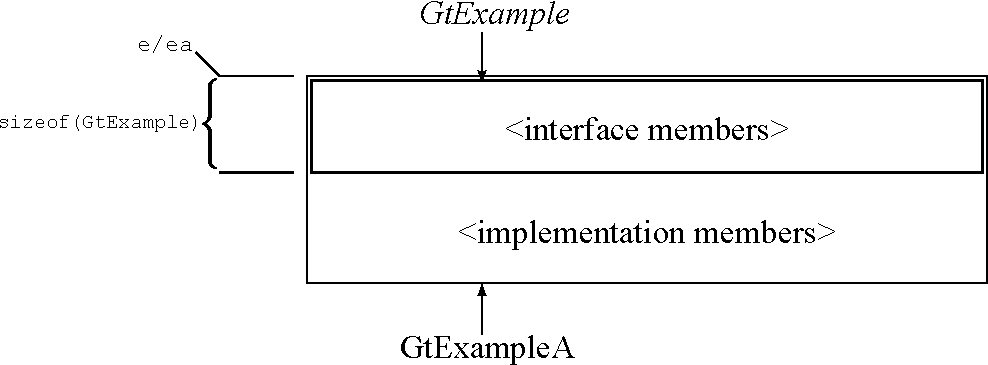
\includegraphics[width=.7\textwidth]{mlayout}
\end{center}
\caption{Memory layout used in the \keyword{GtExampleA} object starting at the
 memory location \keyword{e} implementing the \keyword{GtExample} interface.}
\label{fig:interfacememlayout}
\end{figure}

In the rest of \keyword{example_a.c}, we then code our implementation of the
\keyword{run} interface method:

\begin{lstlisting}
static int gt_example_a_run(GtExample *e) /* hidden from outside  */
{
  GtExampleA *ea = (GtExampleA*) e;       /* downcast to specific type */
  printf("%lu", ea->my_property);         /* run functionality */
  return 0;
}
\end{lstlisting}

Note that we cast our generic \keyword{GtExample*} pointer into a more specific
\keyword{GtExampleA*} pointer. We can do this because we can now be sure that
this function has been called on an object of the \keyword{GtExampleA} class.

We can be sure because we have registered this method as an implementation of
the \keyword{run} interface method by assigning it to the function pointer
variable in the \keyword{GtExampleClass} structure:

\begin{lstlisting}
/* map static local method to interface */
const GtExampleClass* gt_example_a_class(void)
{
  static const GtExampleClass ec = { sizeof (GtExampleA),
                                     gt_example_a_run,
                                     NULL };
  return &ec;
}
\end{lstlisting}

Note that we assign NULL to the \keyword{delete} function slot, because we do
not allocate any memory inside the implementing class we need to free later.
Have a look at the \keyword{example_b.*} files in the \Gt source distribution
for an alternative implementation which allocates additional memory.

We can then use the \keyword{GtExampleClass} returned by this function to write
the \keyword{GtExampleA} constructor, which uses \keyword{gt_example_create()}
to allocate the needed space, initializes the private members and returns the
object:

\begin{lstlisting}
GtExample* gt_example_a_new(void)
{
  GtExample *e = gt_example_create(gt_example_a_class());
  GtExampleA *ea = (GtExampleA*) e;       /* downcast to specific type */
  ea->my_property = 3;                    /* access private implementation
                                             member */
  return e;
}
\end{lstlisting}

Now consider another implementation, \keyword{GtExampleB} which also implements
this interface by creating a \keyword{GtExampleClass} with different implementation-
specific function pointers (see the \keyword{example_b.*} files in the
distribution).

Combining these implementation with the interface headers now allows us to do
the following:

\begin{lstlisting}
#include "example.h"       /* include the interface header */
#include "example_a.h"     /* include the implementation header */
#include "example_b.h"     /* include another implementation header */

int main(int argc, char *argv[])
{
  GtExample *my_e = gt_example_a_new();       /* create GtExampleA object, but
                                                 with interface type */
  gt_example_run(my_e);                       /* call an interface method */
  gt_example_delete(my_e);

  GtExample *my_e = gt_example_b_new();       /* create GtExampleB object, but
                                                 with interface type */
  gt_example_run(my_e);                       /* call an interface method */
  gt_example_delete(my_e);

  return 0;
}
\end{lstlisting}

That is, we can access two implementations via a common set of interface
methods.

\subsection{Modules}

Modules bundle related functions which do not belong to a class. Examples:
\begin{itemize}
\item
\keyword{dynalloc.h}, the low level module for dynamic allocation,
e.g.\ used to implement arrays in \keyword{array.c} and the
above-mentioned strings
\item
\keyword{sig.h}, bundles signal related functions (high level)
\item
\keyword{xansi.h}, contains wrappers for the standard ANSI C library
\item
\keyword{xposix.h}, contains wrappers for POSIX functions we use
\end{itemize}

When designing new code, it is not very often the case that one has to introduce
new modules. Usually defining a new class is the better approach.

\subsection{Unit tests}

Classes and modules should contain a \keyword{gt_<classname>_unit_test} function
which performs a unit test of the class/module and returns 0 in case of success
and -1 in case of failure. More information about how to write unit tests can
be found in section~\ref{unittests}.

\subsection{Tools}

A \emph{tool} is the most high-level type of component \Gt has to offer. Tools
are command line interface (CLI) applications linked into the single \keyword{gt}
binary. They make use of helper classes like the \keyword{GtOptionParser} to
make development of command line tools easier. Having a common interface for
option parsing and error reporting ensures a consistent user experience across
all \Gt tools, as they behave the same way when invoked from the command line.

There are two possible code paths for defining and implementing a tool; only
the newer approach will be described here.
Simply put, a tool is just another object which needs to implement a special
interface, providing callbacks for the \Gt runtime to call at predefined times
during the tool's invocation. An example for a simple tool can
be found in the \keyword{tools} subdirectory in the \keyword{gt_template.[ch]}
files.

First, a tool needs to define a structure to store its arguments. That is,
every command line parameter needs to be represented by a member in the struct
to store its value. For example, for a tool taking a boolean and a string
parameter, we would need the following:

\begin{lstlisting}
typedef struct {
  bool bool_option;
  GtStr  *str_option;
} ExampleToolArguments;
\end{lstlisting}

The tool also requires an initializer function which prepares the argument
structure for value assignment. For example, the \keyword{GtStr} in above
example must be instantiated:

\begin{lstlisting}
static void* gt_example_tool_arguments_new(void)
{
  ExampleToolArguments *arguments = gt_calloc(1, sizeof *arguments);
  arguments->str_option = gt_str_new();
  return arguments;
}
\end{lstlisting}

as well as a destructor function which deletes the argument objects, if
necessary, and then frees the memory used for the argument struct:

\begin{lstlisting}
static void gt_example_tool_arguments_delete(void *tool_arguments)
{
  ExampleToolArguments *arguments = tool_arguments;
  if (!arguments) return;
  gt_str_delete(arguments->str_option);
  gt_free(arguments);
}
\end{lstlisting}

The argument structure is filled by an \emph{option parser}. An option parser
is an object which gets passed an argument list, identifying parameter names
and values and assigning them to the correct variables. It also handles
the creation of a convenient help output by documenting the purpose of each
option and its valid value range. See the interface documentation in
\keyword{src/core/option.h} for a list of possible option types.
A tool must contain a function returning an option parser object:

\begin{lstlisting}
static GtOptionParser* gt_example_tool_option_parser_new(void *tool_arguments)
{
  ExampleToolArguments *arguments = tool_arguments;
  GtOptionParser *op;
  GtOption *option;
  gt_assert(arguments);

  /* initialize with one-liner */
  op = gt_option_parser_new("[option ...] [file]",
                            "This is an example tool for demonstration "
                            "purposes.");

  /* -bool */
  option = gt_option_new_bool("bool",
                              "this is the boolean option",
                              &arguments->bool_option,
                              false);        /* default value */
  gt_option_parser_add_option(op, option);

  /* -string */
  option = gt_option_new_string("string",
                                "pass any string here",
                                arguments->str_option,
                                NULL);       /* default value */
  gt_option_parser_add_option(op, option);

  return op;
}
\end{lstlisting}

The option parser already performs initial validation of the parameters. For
example, it makes sure that a numeric parameter is not given a string value,
that unsigned values are always positive or that probabilities stay between 0
and 1.
In an error case, tool invocation is stopped and the appropriate error message
is printed to \keyword{stderr}.

For more sophisticated error checking, for example involving several parameters
and their values at once, is is possible to write an argument checking function,
which can set an error message in a \keyword{GtError} object (see~\ref{errors})
and return a non-zero return value if an error was found:

\begin{lstlisting}
static int gt_example_tool_arguments_check(GT_UNUSED int rest_argc,
                                           void *tool_arguments,
                                           GT_UNUSED GtError *err)
{
  ExampleToolArguments *arguments = tool_arguments;
  int had_err = 0;
  gt_error_check(err);
  gt_assert(arguments);

  /* we assume that the string parameter must not be empty */
  if (gt_str_length(arguments->str_option) == 0) {
    gt_error_set(err, "parameter 'string' must not be empty!");
    had_err = -1;
  }

  return had_err;
}
\end{lstlisting}

In most cases, however, this function is not necessary and needs not be
implemented.

The most important function which must be implemented in a tools is the runner.
The runner calls the code that actually performs the tool's function and is the
equivalent to the \keyword{main} function in a traditional C program.
Its signature is very similar to a typical C \keyword{main} function as well,
being passed the number of arguments \keyword{argc} and an array of argument
strings \keyword{argv}.:

\begin{lstlisting}
static int gt_example_tool_runner(int argc, const char **argv,
                                 int parsed_args,
                                 void *tool_arguments,
                                 GT_UNUSED GtError *err)
\end{lstlisting}

In addition, it receives the number of arguments (\keyword{parsed_args}) which
were already parsed by the option parser, thus specifying an offset in the
argument array from which the rest of the arguments begin.
That is, if the parameter string was

\begin{lstlisting}
-bool true -string foo bar baz
\end{lstlisting}

then  \keyword{parsed_args} would be 4, as the \keyword{-bool} and
\keyword{-string} options and their values have already been parsed,
leaving \keyword{argv[parsed_args] = 'bar'} and
\keyword{argv[parsed_args+1] = 'baz'} to be handled by the runner.

The rest of the runner function could look like this:

\begin{lstlisting}
static int gt_example_tool_runner(int argc, const char **argv,
                                 int parsed_args,
                                 void *tool_arguments,
                                 GT_UNUSED GtError *err)
{
  ExampleToolArguments *arguments = tool_arguments;
  int had_err = 0;
  gt_error_check(err);
  gt_assert(arguments);

  if (arguments->bool_option)
    printf("the bool option was set\n");
  printf("the string was '%s', gt_str_get(arguments->bool_option));

  return had_err;
}
\end{lstlisting}

Finally, the functions described above are registered in the new tool object
by using \keyword{gt_tool_new()} to create a new \keyword{GtTool} instance
passing pointers to all the static callback functions.

\begin{lstlisting}
GtTool* gt_example_tool(void)
{
  return gt_tool_new(gt_example_tool_arguments_new,
                     gt_example_tool_arguments_delete,
                     gt_example_tool_option_parser_new,
                     gt_example_tool_arguments_check,
                     gt_example_tool_runner);
}
\end{lstlisting}

Let's assume that we have saved the implementation above in
\keyword{tools/gt_example_tool.c}. We then make the \keyword{gt_example_tool()}
function public by adding a \keyword{tools/gt_example_tool.c} header:

\begin{lstlisting}
#ifndef GT_EXAMPLE_TOOL_H
#define GT_EXAMPLE_TOOL_H

#include "core/tool_api.h"

/* the example tool */
GtTool* gt_example_tool(void);

#endif
\end{lstlisting}

This function can then be added to the \Gt toolbox by adding the following lines
to \keyword{gtt.c}:

\begin{lstlisting}
...
#include "tools/gt_example_tool.h"
...
GtToolbox* gtt_tools(void)
{
  ...
  gt_toolbox_add_tool(tools, "example", gt_example_tool());
  ...
}
\end{lstlisting}

After compilation, we can then run our tool by calling

\begin{lstlisting}[language=sh]
$ gt example -bool true -string foo bar baz
\end{lstlisting}%$

\section{Directory structure}
All of these directories are given as subdirectories of the root directory of
the \Gt source distribution.
\begin{itemize}
\item[\texttt{bin/}] This subdirectory contains the \Gt binary executable \texttt{gt}
     as dynamic and static variants as well as the example executables built
     from \texttt{src/examples}. This directory is only populated after a
     make run. Running \texttt{make cleanup} will remove its contents.
\item[\texttt{doc/}] This subdirectory contains documentation such as this
     developer's guide, license information, format specifications, and the
     user manuals for the software tools included with the \Gt .
\item[\texttt{gtdata/}]
     This subdirectory contains data needed for the \Gt to run which are not
     compiled into the \Gt binary itself, such as
     \begin{itemize}
       \item texts for the tool on-line help (in \texttt{gtdata/doc}),
       \item Lua code for documentation generation (in \texttt{gtdata/modules}),
       \item ontology definition files (in \texttt{gtdata/obo\_files}),
       \item \emph{AnnotationSketch} default (e.g.\ a default style file, in
              \texttt{gtdata/sketch}), and
       \item alphabet definition files for character mappings
             (in \texttt{gtdata/trans}).
     \end{itemize}
\item[\texttt{gtpython/}]
     This subdirectory contains the Python bindings to selected parts of the \Gt
     library, as well as the Python test suite. See the \texttt{README} file in
     this directory for installation instructions.
\item[\texttt{gtruby/}]
     This subdirectory contains the Ruby bindings to selected parts of the \Gt
     library. See the \texttt{README} file in this directory for installation
     instructions.
\item[\texttt{gtscripts/}]
     This subdirectory contains a number of Lua scripts written using the \Gt
     Lua bindings; most prominently the \texttt{gtdoc.lua} script to generate
     the documentation. These scripts can be run using the \texttt{gt}
     executable, which is a Lua interpreter as well, by giving the script name
     instead of a tool name.
\item[\texttt{lib/}]
     This subdirectory contains the \Gt static and dynamic libraries when built.
\item[\texttt{obj/}]
     This subdirectory contains object files as they are created during \Gt
     compilation.
\item[\texttt{scripts/}]
     This subdirectory contains useful scripts for \Gt developers.
\item[\texttt{src/}]
     This subdirectory contains the main \Gt source tree. In particular, there
     is a number of subdirectories:
     \begin{itemize}
       \item the \texttt{src/annotationsketch} subdir contains
             \emph{AnnotationSketch} code for genome annotation drawing,
       \item the \texttt{src/core} subdir contains general code, i.e.\
             basic data structures, memory management, file access, encoded
             sequences, sequence parsers, tool runtime, option parser,
             multithreading, etc.,
       \item the \texttt{src/examples} subdir contains simple example
             applications built on \Gt (streams, or a GUI app),
       \item the \texttt{src/extended} subdir contain code for annotation
             handling and parsing, stream processing, alignment, chaining, etc.,
       \item the \texttt{src/external} subdir contains third-party source code
             which is distributed with the \Gt source and built alongside the
             \Gt ,
       \item the \texttt{src/gth} subdir with \emph{GenomeThreader} code,
       \item the \texttt{src/gtlua} subdir with Lua bindings for some of the \Gt
             classes and modules,
       \item the \texttt{src/ltr} subdir with LTR retrotransposon prediction and
             annotation code,
       \item the \texttt{src/match} subdir with code for index structure
             construction and access, short read mapping, matching algorithms
             etc.,
       \item the \texttt{src/mgth} subdir contains \emph{MetaGenomeThreader}
             code,
       \item the \texttt{src/patches} subdirectory with platform-specific
             patches, and
       \item the \texttt{tools} subdir with code for all the tools included with
             \Gt .
     \end{itemize}
\item[\texttt{testdata/}]
     This subdirectory contains test data used in the testsuite. Please refrain
     from storing large files ($>1$MB) in this directory, but use the
     \keyword{gttestdata} repo instead (see~\ref{gttestdata}). Special
     subdirectories:
     \begin{itemize}
       \item The \texttt{testdata/gtscripts} subdir contains test scripts used
       in the Lua test cases,
       \item the \texttt{testdata/gtruby} subdir contains test scripts used
       in the Ruby test cases, and
       \item the \texttt{testdata/gtpython} subdir contains test scripts used
       in the Python test cases.
     \end{itemize}
\item[\texttt{testsuite/}]
     This subdirectory contains the test suite definitions as Ruby files as
     well as the test engine and temporary data created using test runs.
     After starting a test suite run, the \keyword{testsuite/stest_testsuite}
     subdirectory then contains a directory named \keyword{test<n>} for each
     test, where \keyword{<n>} is the test number. See~\ref{testdefinitions}
     for more details.
\item[\texttt{www/}]
     This subdirectory contains the content of the \Gt website.
\end{itemize}


\section{Public APIs}

In \Gt , we distinguish between \emph{public} and \emph{non-public} application
programming interfaces (APIs). The API describes the classes and modules
belonging to the \Gt and their methods and functions, in particular their
signatures; that is, their name, return value, and number and types of their
parameters.

The public API is a subset of the \Gt library which is intended to be used by
developers which do not belong to the \Gt core development team, and is fairly
high-level at this point. To ensure compatibility with future versions of the
\Gt library, the public API is supposed to be subject to as little change as
possible. That is, interface changes should be made very sparsely, and interface
design should `look forward' to make such changes unneccessary. For example,
interface functions which could fail in theory should receive error handling
facilities in their signature (such as a return code and a \keyword{GtError}
object), even if their current (and maybe only) implementation cannot fail. This
leaves room for implementations that \emph{may} fail without having to break the
API when the new implementation finds its way into the \Gt .

All public API functions for a given class must be declared in a prototype
header file named \keyword{<class>_api.h}. This header file must only include
other public API headers. All of the public API header files are packaged to be
distributed with the \Gt tarball and are installed into the given include path.
That is, the functions defined in them are later accessible by including
\keyword{genometools.h} only.

It is important to note that all functions in the public header files must be
properly documented (see section~\ref{documentation}).

\section{Coding style}

\subsection{General rules}
\begin{itemize}
\item
No line in the source code must be longer than 80 characters.
This allows proper formatting of the code.
\item
There must be not more than one consecutive empty line in the source code.
\item
Trailing spaces are disallowed.
\item
There must not be a comma at the beginning of a line.
\item
Unless it is at the end of a line, a comma should be followed by a space.
Example:

\begin{lstlisting}
cmpfunc(gt_array_get(a, idx), gt_array_get(b, idx));
\end{lstlisting}

instead of

\begin{lstlisting}
cmpfunc(gt_array_get(a,idx),gt_array_get(b,idx));
\end{lstlisting}

\item
The symbols `\keyword{=}', `\keyword{==}' und `\keyword{!=}' should be
enclosed by spaces. That is, write

\begin{lstlisting}
i = 0;
\end{lstlisting}

instead of

\begin{lstlisting}
i=0;
\end{lstlisting}
\item
There must be a space between the keywords \keyword{for}, \keyword{if},
\keyword{sizeof}, \keyword{switch}, \keyword{while} and \keyword{do} and the
following parenthesis.
\item
The opening braces (\keyword{\{}) after the keywords \keyword{if},
\keyword{else}, \keyword{for}, \keyword{do}, and \keyword{while} should be on
the same line as the keyword.
\item
The curly braces following an \keyword{if} or \keyword{else} expression should
be omitted if the expression and the (single) following statement both fit on
a single line.
\item
The keyword \keyword{else} should be placed on a separate line.
\item
Semantic blocks (statements inside loops, function definitions, etc.) must be
indented by exactly two spaces w.r.t.\ the enclosing block.
This explicitly means \emph{no tabs}, configure your editor!

Here is an example:
\begin{lstlisting}
bool
gt_array_equal(const GtArray *a, const GtArray *b, GtCompare cmpfunc)
{
  unsigned long idx, size_a, size_b;
  int cmp;
  gt_assert(gt_array_elem_size(a) == gt_array_elem_size(b));
  size_a = gt_array_size(a);
  size_b = gt_array_size(b);
  if (size_a < size_b)
    return false;
  if (size_a > size_b)
    return false;
  for (idx = 0; idx < size_a; idx++) {
    cmp = cmpfunc(gt_array_get(a, idx), gt_array_get(b, idx));
    if (cmp != 0)
      return false;
  }
  return true;
}
\end{lstlisting}
\item
Use the \keyword{scripts/src_check} and \keyword{scripts/src_clean} scripts
regularly to check your source code for style violations.
\item
Use the \keyword{scripts/pre-commit} git hook to automatically run a
\keyword{src_check}
before each commit. The commit will be canceled if errors are found.\\
To enable the git hook, copy the file \keyword{scripts/pre-commit} into the
\keyword{.git/hooks} subdirectory of your \Gt repository.
\item
Static variables inside functions are not allowed. An exception are class
structs, which must be static.
\item
All functions except those which should be callable publicly should be declared
as \keyword{static}. All non-static functions must be documented in a
header file.
Think twice before making a function public. Its interface should be clean
enough to be understood by someone who does not know implementation details!
\item
If a \Gt module or class exists for your particular need, use it instead of
using more low-level means (e.g.\ try to use \keyword{GtFile} and friends for
file access instead of \keyword{fopen()}/\keyword{fclose()}/\dots\ directly).
Consult the documentation and the header files!
\end{itemize}

\subsection{Global variables}
\begin{itemize}
\item
Generally, global variables are not allowed.
\item
There are exceptions in very rare cases, in which must be made sure that the
content in question is initialized, synchronized for multithreaded use and
properly cleaned up. Do not add global variables without talking to one of the
core developers!
\end{itemize}

\subsection{Types}
\begin{itemize}
\item
Use unsigned types whereever possible. We need to process large amount
of data and we may need every bit to process it.
\item
Use \keyword{unsigned long} for sequence positions/lengths/offsets/\dots .
The \keyword{unsigned long} type equals the word size on all common systems
(i.e., it is 32-bit wide on 32-bit systems and 64-bit wide on 64-bit systems)
which makes it ideal for most use cases.
\item
Use \keyword{GtStr} and \keyword{GtArray} instead of manipulating byte arrays
directly if possible, especially when returning strings or item collections
from a function.
\end{itemize}

\subsection{Naming rules}
\begin{itemize}
\item
Class names must begin with \keyword{Gt}, e.g. \keyword{GtArray},
\keyword{GtNodeStream}.
\item
Class names may use camel
case\footnote{\url{http://en.wikipedia.org/wiki/CamelCase}} if multiple words
are required, e.g.\ \keyword{GtNodeStream}.
\item
Source and header files for a class must start with the class name in
lowercase, without the \keyword{Gt} prefix. If camel case is used in the class
name, use underscores in the respective file name, e.g.\
\keyword{GtNodeStream} $\to$ \keyword{node_stream.[ch]}.
\item
Variable names and function names must be all lower-case.
\item
Variable names and function names should use underscores to separate words
(e.g. use the function name \keyword{get_first_five_chars} instead of
\keyword{getfirstfivechars}).
\item
The names of public (i.e.\ non-static) functions must be prefixed by the string
`\keyword{gt_}' to avoid namespace clashes when linking the \Gt library with
third-party code.
\item
Class or module names must follow the `\keyword{gt_}' part in the function name.
\item
In method signatures, the object on which the method is called must always be
the first argument of the method.
That is, method \keyword{method} in class \keyword{GtClass} must be defined as:
\begin{lstlisting}
<type> gt_class_method(GtClass*, <params>);
\end{lstlisting}
\end{itemize}

\subsection{Copyright lines}
\label{copyright}
\begin{itemize}
\item
Every header and C source file must begin with a comment containing author and
license information:
\begin{lstlisting}
/*
Copyright (c) 2007-2010 Gordon Gremme <gordon@gremme.org>
Copyright (c) 2007-2008 Center for Bioinformatics, University of Hamburg

Permission to use, copy, modify, and distribute this software for any
purpose with or without fee is hereby granted, provided that the above
copyright notice and this permission notice appear in all copies.

THE SOFTWARE IS PROVIDED "AS IS" AND THE AUTHOR DISCLAIMS ALL WARRANTIES
WITH REGARD TO THIS SOFTWARE INCLUDING ALL IMPLIED WARRANTIES OF
MERCHANTABILITY AND FITNESS. IN NO EVENT SHALL THE AUTHOR BE LIABLE FOR
ANY SPECIAL, DIRECT, INDIRECT, OR CONSEQUENTIAL DAMAGES OR ANY DAMAGES
WHATSOEVER RESULTING FROM LOSS OF USE, DATA OR PROFITS, WHETHER IN AN
ACTION OF CONTRACT, NEGLIGENCE OR OTHER TORTIOUS ACTION, ARISING OUT OF
OR IN CONNECTION WITH THE USE OR PERFORMANCE OF THIS SOFTWARE.
*/
\end{lstlisting}
\item
Each developer with substantial contributions (for example, by implementing new
features, refactoring, or fixing bugs which require large rewrites) should
give his/her name and email address, updating the given year ranges in the
process.
\item The "Center for Bioinformatics" copyright line is only required for
developers employed by it, because only in this case the University gains any
copyright.
\end{itemize}

\subsection{Header files}
\begin{itemize}
\item
Use conditional inclusion to avoid including the same header file multiple
times. Between the copyright header and the beginning of the declarations, put
the following:
\begin{lstlisting}
#ifndef FILENAME_H
#define FILENAME_H
\end{lstlisting}
and put an
\begin{lstlisting}
#endif
\end{lstlisting}
at the end of the header file.
This causes the preprocessor to include the section between the
\keyword{#ifndef} and \keyword{#endif} only once.
\item
The identifier to be \keyword{#define}d must be the filename of the header
file in uppercase with all non-alphanumeric characters replaced by underscores.
\end{itemize}

\subsection{Comments and documentation}
\label{documentation}
\begin{itemize}
\item
Comments are written in plain C style (\keyword{/* ... */}). C++-style
comments (\keyword{// ...}) are disallowed.
\item
The public API files (header files ending in \keyword{*_api.h}) are examined for
automatic generation of API documentation. The following annotations are
supported:
\begin{itemize}
\item
Each type (e.g.\ class) should be directly preceded by a comment describing the
purpose of the class. Example:

\begin{lstlisting}
/* <GtArray*> objects are generic arrays for elements of a certain
   size which grow on demand. */
typedef struct GtArray GtArray;
\end{lstlisting}

\item
Each function (method) should be directly preceded by a comment describing the
purpose of the function, its preconditions, return value, and parameters.
Example:

\begin{lstlisting}
/* Add element <elem> to <array>. The size of <elem> must equal the
   given element size when the <array> was created and is determined
   automatically with the <sizeof> operator. */
#define       gt_array_add(array, elem) \
              gt_array_add_elem(array, &(elem), sizeof (elem))
/* Add element <elem> with size <size_of_elem> to <array>.
   <size_of_elem> must equal the given element size when the <array>
   was created. Usually, this method is not used directly and the
   macro <gt_array_add()> is used instead. */
void          gt_array_add_elem(GtArray *array, void *elem,
                                size_t size_of_elem);
\end{lstlisting}
\item
Code keywords (parameters, class names, references to other functions) can be
marked by putting them between angled brackets (\keyword{<}\dots\keyword{>}).
Also, keywords can be marked as strong (bold) by putting them between
three underscores (\keyword{___}\dots\keyword{___}) or emphasized (italic) by
using two underscores (\keyword{__}\dots\keyword{__}).
\end{itemize}
\item
The comment line should briefly describe
\begin{itemize}
\item
what the method does (e.g.\ ``Calculates and returns X\dots'',
``Delivers the next element in order\dots'', ``Adds element X\dots''),
\item
what \emph{all} parameters are supposed to be (ideally given in the context of
what the method does),
\item
what the return value is,
\item
potential side-effects, and
\item
if the function receives or returns a pointer, whether ownership is taken or
retained for the accepted or returned memory (i.e.\ ``takes ownership of
parameter X'' or ``X must be deleted by the caller'').
\end{itemize}
\item
Do not group multiple functions beneath one comment line, even if they are
largely similar and differ only in minor details. If required, repeat the
comment above each function to ensure that both get an entry in the generated
documentation.
\item
Stars (\keyword{*}) are \emph{not} to be continued on every line of the comment,
as many editors like to do by default. Doing so anyway will lead to interspersed
star symbols in the generated output.
\item
Please refrain from using other markup formats such as Doxygen or Javadoc style.
It may look alright in the plain text, but will most certainly come out weird in
the generated LaTeX or HTML documents.
\item
Use the \keyword{docs} target in the \Gt Makefile to build the API
documentation, which is then found in \keyword{www/genometools.org/htdocs}
subdirectory (libgenometools.html).
\end{itemize}

\subsection{Function pointers}
\begin{itemize}
\item
Function pointer declarations used in public headers (e.g.\ to be used as method
arguments) should always be \keyword{typedef}'ed to an identifier prefixed with
\keyword{Gt}. An example:
\begin{lstlisting}
typedef int  (*GtCompareWithData)(const void*, const void*, void *data);
\end{lstlisting}

The function pointer type can then be used in a sort function this way:

\begin{lstlisting}
void gt_qsort_r(void *a, size_t n, size_t es, void *data,
                GtCompareWithData cmp);
\end{lstlisting}

instead of:

\begin{lstlisting}
void gt_qsort_r(void *a, size_t n, size_t es, void *data,
                int (*cmp)(const void*, const void*, void *data));
\end{lstlisting}

which makes the headers much harder to read.
\item
If callback functions need additional data to work, provide an additional
\keyword{void*} pointer to pass external data to the callback function
(as, for example, done with the \keyword{data} parameter in the function
\keyword{gt_qsort_r()} above). Do not use global variables for that purpose!
\end{itemize}

\subsection{\texttt{\#define}s}
\begin{itemize}
\item
Identifiers introduced by a \keyword{\#define} statement should be completely
written in upper case letters. This also holds for the arguments of
macros.
\item
Identifiers introduced by public \keyword{\#define}s should be prefixed with
\keyword{GT_}.
\item
In public headers, \keyword{\#define} statements should only set constants.
Macros defining code parts should only be used -- very sparingly -- locally
within a class or module implementation.
\end{itemize}

\subsection{Information hiding}
In \Gt, we try to adhere to object-oriented design guidelines. An integral
part of these is the enforcement of \emph{information hiding} or
\emph{encapsulation}, that is, making access to an object's internal state
only possible through accessor functions.

From this, it follows directly that the use of `open' structs, that is, C
structures defined in public headers, is strongly discouraged! Structures (and
structure member accesses) should only be implemented within a C file. This
applies to both structures used to implement classes as well as structures used
as auxiliary data structures.

A notable exception are structs implementing classes which only act as
containers, i.e.\ in which the only methods manipulating the members would be
setter and getter methods (see \keyword{core/range_api.h}).
However, even those structures should provide accessor, constructor and
destructor methods so they can safely be created, accessed and deleted from
scripting language bindings lacking support for proper C structure access.



\section{Error handling}
We distinguish between \emph{programming errors} and \emph{run-time errors}.
Programming errors occur when the developer uses resources in an inherently
erroneous way, e.g.\ passing a null pointer where a valid pointer is expected,
passing incorrect length values to string comparison functions, or accessing
uninitialised memory. This often happens because of incomplete documentation,
or by running into ``corner cases'' which were overlooked. If undetected, they
can lead to nasty bugs that are hard to track down.

Other special cases are expected to come up sooner or later. For example, a user
may specify a file name for input or output which is not readable or writable,
or which does not exist. Typically, it is not intended to terminate program
execution at that point, but to react in a graceful way (e.g.\ by creating a new
file, reporting a proper error message, or asking for a different file name).
These are run-time errors.

\subsection{Programming errors}
\begin{itemize}
\item
Use \keyword{gt_assert()} to check invariants in your program, that is, any
conditions that you hold to be true for the following code to work properly.
For example, in a function getting a pointer as a parameter which is to be
dereferenced later, you should assert that the pointer is not \keyword{NULL}
prior to dereferencing.
Similarly, in a function that is supposed to never return a negative number,
one should use \keyword{gt_assert()} to check this condition directly before the
\keyword{return} statement.
\item
If the expression given to \keyword{gt_assert()} as a parameter evaluates to
\keyword{false} (that is, 0, \keyword{false}, or \keyword{NULL}), the program
will abort.
\item
Assertions can be disabled at compile time by passing the \keyword{assert=no}
switch to the \keyword{make} call. If variables or parameters are only used in
an assertion, disabling assertions may trigger this error message:
\begin{lstlisting}
error: unused parameter 'x'
\end{lstlisting}
or
\begin{lstlisting}
error: unused variable 'y'
\end{lstlisting}
Include \keyword{core/unused_api.h} and prefix the declaration of the offending
identifier with \keyword{GT_UNUSED} to inform the compiler that this variable is
intentionally unused.
\end{itemize}

\subsection{Run-time errors}
\label{errors}
\begin{itemize}
\item
Functions that are allowed to fail at run-time must return a negative error
code or \texttt{NULL}. The code for successful execution should be 0 or a
pointer different from \texttt{NULL}. Positive return values may be used as
results.
Such functions should also receive a \keyword{GtError} object as their last
parameter, in order to store and propagate error messages.
If a function may return an error code or \texttt{NULL}, \emph{always} check for
this and handle the case accordingly.
\item
Use the \keyword{GtError} class (see \keyword{core/error_api.h}) for storing
error messages and error status:
\begin{lstlisting}
char* get_first_five_chars(const char *str, GtError *err)
{
  char *ret;
  if (strlen(str) < 5) {
    gt_error_set(err, "string '%s' is shorter than 5 characters", str);
    return NULL;
  }
  ret = gt_calloc(6, sizeof (char));
  strncpy(ret, str, 5);
  return ret;
}
\end{lstlisting}
\item
Use a variable called \keyword{had_err} which is initialized to 0 and then
assigned an error status such that an error is set when \keyword{had_err}$\neq 0$:
\begin{lstlisting}
int had_err = 0;
const char *prefix;
GtError *err = gt_error_new();
if ((prefix = get_first_five_chars("foo", err))) {
  /* go on with next step */
}
else
  had_err = -1;
if (!had_err) {
  ...
}
\end{lstlisting}
\keyword{-1} should be used to store an error in the \keyword{had_err} variable.
It is very idiomatic to write \keyword{if (had_err)...} or
\keyword{if (!had_err)...}.
\item
Catch run-time errors and create error messages as close to their source as possible.
\item
The error object should always be the last parameter and should be named
\keyword{err}.
\end{itemize}

\section{Memory management}
\subsection{Allocation/deallocation}
\begin{itemize}
\item
Space allocation is only allowed using the \keyword{gt_malloc()},
\keyword{gt_calloc()}, \keyword{gt_realloc()} functions in
\keyword{core/ma_api.h}. Use \keyword{gt_free()} to deallocate memory.
These methods are analog to \keyword{malloc(3)}, \keyword{calloc(3)} and
\keyword{realloc(3)} from the C standard library, except that they never return
\keyword{NULL} upon failure.
\item
The \keyword{gt_ma_get_space_peak()}, \keyword{gt_ma_show_space_peak()} and
\keyword{gt_ma_check_space_leak()} functions in \keyword{core/ma_api.h} can be
used to evaluate memory usage and check for memory leaks.
\end{itemize}

\subsection{Reference counting}
Sometimes it is desired to have an object referenced by more than one other
object, avoiding to \keyword{gt_free()} the object's memory until the last
reference to the object has been dropped. In \Gt, \emph{reference counting} is
used to implement this behaviour. That is, each object keeps the number of
objects still keeping a reference on it in a local member variable. This is done
by each referencing object calling the object's \keyword{ref()} method to
announce that they now keep a reference, thus increasing the reference count.
When the object reference is no longer needed, the usual \keyword{delete()}
method is used. The \keyword{delete()} method checks and decreases the
reference count and defers free'ing the object's memory until the object is not
referenced by any other object any more. This makes reference counting a simple
form of garbage collection.

To add reference counting to a class, perform the following steps:
\begin{itemize}
\item Add an \keyword{unsigned int} counter variable called
\keyword{reference_count} to the private member variables of the class; this
variable must be initialized to 0 in the constructor.
\item Consider a class \emph{GtFoo} to which we want to add reference counting
capabilities. Then add a method \keyword{gt_<classname>_ref()}, in this case
\keyword{gt_foo_ref()} to the interface of the class:

\begin{lstlisting}
GtFoo* gt_foo_ref(GtFoo *f)
{
  gt_assert(f);
  f->reference_count++;
  return f;
}
\end{lstlisting}

\item
In the destructor, check the reference count and only free the memory when
necessary:

\begin{lstlisting}
void gt_foo_delete(GtFoo *f)
{
  if (!f) return;
  if (f->reference_count) {
    f->reference_count--;
    return;
  }
  gt_free(f);
}
\end{lstlisting}

\end{itemize}

With reference counted classes, always use the \keyword{ref()} method when
storing a reference to an object. That is, instead of writing

\begin{lstlisting}
void gt_bar_set_foo(GtBar *b, GtFoo *f)
{
  b->value = f;
}
\end{lstlisting}

use

\begin{lstlisting}
void gt_bar_set_foo(GtBar *b, GtFoo *f)
{
  b->value = gt_foo_ref(f);
}
\end{lstlisting}

Always remember to call \keyword{gt_foo_delete()} when the reference is
no longer needed! For example, in the assignment above, a good place to do this
is the destructor of the \keyword{GtBar} class.

\subsection{Library initialization/finalization}
Within the \Gt code, there are a number of global or static data which must be
properly initialized before using any \Gt functionality, and space for which
must be properly freed when done using the \Gt . This is usually done by the
runtime by calling initializers when a tool is run using the \keyword{gt}
binary.

Now consider that \Gt can also be used as a library, called
\keyword{libgenometools}. That means, it is possible to link an external code
with the static or shared object file and call functions from there, without
going through the tool runtime. It is now crucial that the necessary
initializations have taken place before using functions, and that the required
cleanup is done at the end.

There are two functions in the \keyword{core/init.[ch]} module in \Gt used to
accomplish this:
\begin{itemize}
\item
\keyword{gt_lib_init()}, which initializes all static data and should be called
before any other \Gt function, and
\item
\keyword{gt_lib_clean()}, which frees all static data. It returns 0 if no
memory map, file pointer, or memory has been leaked and a value other than 0
otherwise.
\end{itemize}
It is also possible to make the cleanup happen automatically when the program
using  the library exits. This is done by calling
\keyword{gt_lib_reg_atexit_func()} which registers an exit handler with the OS
which will call \keyword{gt_lib_clean()} automatically.

\section{Threads}
The \Gt contain functions allowing developers to write their programs in a
multi-threaded way, by wrapping the POSIX threads library \keyword{libpthread}.
See \keyword{core/thread\_api.h} for more information.

Any function with this signature:

\begin{lstlisting}
void* (*GtThreadFunc)(void *data);
\end{lstlisting}

can be enabled to be run concurrently by simply calling

\begin{lstlisting}
void *mythread(void *data)
{
 ...
}
gt_multithread(mythread, NULL, err);
\end{lstlisting}

Some more useful information:
\begin{itemize}
\item
For synchronization during parallel execution of multiple threads, \Gt provides
classes for mutexes and read-write-locks. See \keyword{core/thread\_api.h} for a
description of the interface of the \keyword{GtMutex} and \keyword{GtRWLock}
classes.
\item
If code must be conditionally compiled depending on thread support, use
\keyword{#ifdef} and friends with the \keyword{GT_THREADS_ENABLED} flag, which
is set by the compiler via a \keyword{-D} option when threading support is
enabled.
\item
Threading support is enabled at compile time by passing \keyword{threads=yes} to
the \keyword{make} call. If threading support is not enabled, all
\keyword{gt_multithread()} functions will run the thread function sequentially.
\item
If threading support is enabled, the number of concurrent jobs can be given
using the \keyword{-j} parameter to the \keyword{gt} binary. That is, to have
all multithreaded parts in the tool to be run use three threads at once, call
the tool with

\begin{lstlisting}
$ gt -j 3 <toolname> ...
\end{lstlisting}%$

\end{itemize}


\section{Testing and Debugging}
\subsection{Testing on the code level -- the unit tests}
\label{unittests}

Unit test check whether classes and their methods behave correctly when used in
a correct manner. The corresponding functions must be defined in the class
implementation file (so they get access to the private member variables of the
tested class) and adhere to the following interface:

\begin{lstlisting}
int  (*UnitTestFunc)(GtError *err);
\end{lstlisting}

They must return 0 if the test was successful and -1 if the test has failed.
The \keyword{gt_ensure} helper macro makes writing unit tests easier. To use it,
\keyword{#include} the file \keyword{core/ensure.h}. Then write your unit test:

\begin{lstlisting}
int gt_class_unit_test(GtError *err) /* must be called 'err'! */
{
  int had_err = 0;                   /* must be called 'had_err'! */
  gt_error_check(err);               /* will abort if error was already set */

  gt_ensure(1 + 1 == 2);    /* will succeed */
  gt_ensure(1 + 1 == 3);    /* will fail */

  return had_err;
}
\end{lstlisting}

Similarly to \keyword{gt_assert()}, if the expression given to
\keyword{gt_ensure()} as a parameter evaluates to false, the test will fail with
an error message, giving the location at which the first condition failed.
Because \keyword{gt_ensure()} is implemented as a macro relying on certain
naming conventions, it is mandatory that the \keyword{int} error indicator
variabel and the \keyword{GtError} object within the test function are called
\keyword{had_err} and \keyword{err}.

The unit tests are added to the test suite in the function
\keyword{gtt_unit_tests()} in \keyword{gtt.c} and loaded into the \Gt runtime
in the function \keyword{gtr_register_components()} in \keyword{gtr.c}.
That is, if your unit test function is \keyword{gt_class_unit_test()}, then you
should \keyword{#include} the header \keyword{class.h} (which contains the
function prototype) in \keyword{gtt.c} and add the following line in
\keyword{gtt_unit_tests()}:
\begin{lstlisting}
gt_hashmap_add(unit_tests, "example class", gt_class_unit_test);
\end{lstlisting}

The tests registered in this hash table can be executed on the command line
with:

\begin{lstlisting}[language=sh]
$ gt -test
\end{lstlisting}%$

It is also possible to run a single test from the test suite by using the
\keyword{-only} option:

\begin{lstlisting}[language=sh]
$ gt -test -only 'example class'
\end{lstlisting}%$

\subsection{Testing on the tool level -- the test suite}

While the unit tests check the correctness of the classes and modules on the
code level, the Ruby-based test suite is used to run tests on the tools
themselves. That means that they run tools with example data or invalid
parameters and check whether they behave correctly by looking at error levels,
error messages, and comparing output with reference data.

Test data and reference data are stored in the \keyword{testdata/} directory
of the \Gt source tree. Note that this directory is for smaller test data only.
Large files, such as whole chromosome annotations go into another repository
(see~\ref{gttestdata}).

\subsubsection{Test definitions}
\label{testdefinitions}

Tests are defined in the \keyword{gt_<toolname>_include.rb} files in the
\keyword{testsuite/} directory. They contain test definitions written in a
Ruby-based domain specific language. Here is an example of a simple test:

\begin{lstlisting}[language=Ruby]
Name "gt cds test (description range)"
Keywords "gt_cds usedesc"
Test do
  run_test "#{$bin}gt cds -usedesc -seqfile " +
           "#{$testdata}gt_cds_test_descrange.fas " +
           "#{$testdata}gt_cds_test_descrange.in"
  run "diff #{$last_stdout} #{$testdata}/gt_cds_test_descrange.out"
end
\end{lstlisting}%$

This test runs the \keyword{gt cds} command with example data and compares its
output on stdout with a reference file.

Every test case must have a \keyword{name} and can have a set of \emph{keywords}
associated with it, allowing for selective running of a subset of tests from
all testsuites. Keywords are separated by spaces.
The actual test code is given in the \keyword{Test} environment.
Within this environment, one may use the following constructs to define test
conditions:

\begin{itemize}
\item
\keyword{run_test(runstring, options)}, where
\begin{itemize}
\item
\keyword{runstring} is the tool commandline to run, and
\item
\keyword{options} are a hash specifying test constraints.
The key \keyword{:retval} specifies the expected error code for this run (0 is
the default). The option \keyword{:maxtime} specifies the maximal time in
seconds that the started program may run before it is killed, resulting in a
failed test (60 is the default). This allows one to detect infinite loops
without stopping the testing progress.
\end{itemize}
This command runs the command specified in \keyword{runstring}, and causes the
test to fail if the returned error code does not equal the expected one.
\item
\keyword{grep(file, pattern)} which searches for \keyword{pattern} in the
file \keyword{file}, failing the test if there is no match. The pattern can be
given as a regular expression.
\item
\keyword{run_ruby(rubyscript, options)} and
\keyword{run_python(pythonscript, options)} can be used to run tests on
external Ruby and Python scripts.
\item
Any Ruby code, such as custom functions, can be run inside the \keyword{Test}
environment. To fail a test case manually, use the \keyword{failtest(msg)}
command, where \keyword{msg} is the error message to fail with.
\end{itemize}
Inside test suite definitions, some useful paths are predefined to be
conveniently used in test runs (like \keyword{$bin} and \keyword{$testdata} in
the example above):
\begin{itemize}
\item
\keyword{$testdata}, the path to the \keyword{testdata/} directory,
\item
\keyword{$gttestdata}, the path to the location of the \keyword{gttestdata}
repository (see~\ref{gttestdata}),
\item
\keyword{$bin}, the path to the \Gt \keyword{bin/} directory,
\item
\keyword{$cur}, the path to the current test case directory (each test is run in
a separate directory),
\item
\keyword{$transdir}, the path to the \keyword{gtdata/trans} directory,
\item
\keyword{$obodir}, the path to the \keyword{gtdata/obo_files} directory,
\item
\keyword{$gtruby}, the path to the \keyword{gtruby/} directory,
\item
\keyword{$gtpython}, the path to the \keyword{gtpython/} directory,
\end{itemize}
It is also possible to get the standard output and standard error contents of
the last command run by referring to the files specified by
\keyword{last_stdout} and \keyword{last_stderr}.

Furthermore, each test commandline (let's say the $i$-th one in the test)
creates a set of \keyword{run_}$i$ (contains the actual command which was run),
\keyword{stdout_}$i$ (contains the standard output) an \keyword{stderr_}$i$
(contains the standard error output) files in the test directory (which is
\keyword{testsuite/stest_testsuite/test}$n$\keyword{/}, where $n$ is the test
number (printed in front of each test name).

\subsubsection{The \keyword{gttestdata} repository}
\label{gttestdata}

Large test or reference data must not be placed into the \Gt \keyword{testdata/}
directory because they would increase the size of the \Gt distribution too much.
For such data there is a separate repository, which is available via Git:

\begin{lstlisting}[language=sh]
$ git clone git://genometools.org/gttestdata.git
\end{lstlisting}%$

The location of the \keyword{gttestdata} repository must be given when running
the testsuite (see below). If it is not given, make sure that test which depend
on large test data are disabled (e.g. by placing them in an
`\keyword{if $gttestdata}' clause).%$

\subsubsection{Running the testsuite}
A comprehensive \Gt test run, containing both the unit tests and the tool tests,
can be initiated by issuing \keyword{make test} in the \Gt directory.
The following \keyword{make} switches influence the test runs:
\begin{itemize}
\item
\keyword{memcheck=yes} enables memory access checking via \emph{valgrind},
\item
\keyword{testthreads=<n>} enables multithreaded testing with \keyword{<n>}
threads in parallel to speed up test runs,
\item
\keyword{testrange=<range>} only runs tests with numbers within the given range,
which has to be given in Ruby Syntax i.e. \keyword{i..j}. It is also possible to
provide a list of numbers (devided by space, so use "" to encapsule).
\item
\keyword{gttestdata=<path>} tells the test suite to look for large test data in
\keyword{<path>}. This must be where a copy of the \keyword{gttestdata}
repository is installed.

\end{itemize}

The tool tests can also be run using the \keyword{testsuite/testsuite.rb}
script. Use the \keyword{-keywords <keywords>} parameter to only run these
tests tagged with the given keywords. OR and AND operators can be used to
specify the tests in a more detailed way. The \keyword{-select <n>} parameter
can be used to run only the one test with number \keyword{n} (use
\keyword{-select <m..n>} for ranges), and the \keyword{-threads <n>} will run
the testsuite with \keyword{n} threads in parallel.

To make tests depending on randomized values reproducible, the test suite will
pick a RNG seed before starting any tests and will run all \keyword{gt}
invocations with the environment variable \keyword{GT\_SEED} set to this seed
value. This seed value is also output by \keyword{testsuite/testsuite.rb}. This
makes sure that all tests are run with a common random seed, instead of picking
a new one each time \keyword{gt} is run in a test.

\subsection{Header inclusion dependencies}
Often function prototypes in the \Gt header files use types declared in
another header files. By mistake, it is possible to forget
\keyword{#include}'ing the header files where the type is defined in the header
using it. Note that this problem may never surface if the forgotten header
is included in every C source file which includes the header file with the
missing include statement. To address this, the script
\keyword{scripts/src_check_header.rb} tries to include each header file given
as a command line argument by itself in a C file and compile it.
If dependencies are missing, the check will abort and output the compiler error
message so the problem can be fixed.

\subsection{Debug symbols}
Compilation with debug symbols is enabled by default.
To make sure that line numbers are correct when using a debugger, e.g.
\keyword{gdb}, use the \keyword{opt=no} option in the \keyword{make} call to
disable compile-time optimization. The \keyword{opt} option is enabled by
default.

\subsection{Profiling}
To enable the generation of profiling output in the compiled binaries, use the
\keyword{prof=yes} option in the \keyword{make} call. The \keyword{prof} option
is disabled by default. Enabling this option makes the \Gt binary create a
\keyword{gmon.out} file during each run, which can then be used for analysis
using \emph{gprof}\footnote{See
\url{http://sourceware.org/binutils/docs/gprof/index.html} for further
information.}.

\subsection{Logging}

Use the \keyword{gt_log_*()} functions in \keyword{core/log_api.h} to log debug
messages to the screen or files. Output of debugging information defined using
these functions can then be enabled or disabled via the \keyword{-debug} option
of the \keyword{gt} binary. That is, to run tool \keyword{mytool} with debug
output enabled, run

\begin{lstlisting}
$ gt -debug mytool
\end{lstlisting}%$

\section{Additional \keyword{make} parameters}

\subsection{Additional targets}
Simply running \emph{make} builds both the \keyword{gt} executable and the
\Gt shared library. However, there are also other targets (besides the ones
mentioned in the respective sections above) which can be built using the \Gt
Makefile:
\begin{itemize}
\item
\keyword{docs}, which builds API documentation as web pages in \keyword{www} and
as \LaTeX\ source in \keyword{doc/},
\item
\keyword{manuals}, which, in addition to the files created by \keyword{docs},
also creates manuals for some published tools in \Gt (see
\keyword{doc/manuals}),
\item
\keyword{install}, which installs the compiled \Gt binaries, libraries and
headers into the directory specified by the \keyword{prefix=<path>} option,
\item
\keyword{dist}, which creates a tarball with a binary \Gt distribution, which
will then reside in the \keyword{dist/} subdirectory of the \Gt root,
\item
\keyword{srcdist}, which creates a tarball with a source \Gt distribution, which
will then reside in the working directory,
\item
\keyword{spgt}, which checks selected files in the \keyword{core/} and
\keyword{match/} subdirectories using the splint static
checker\footnote{\url{http://www.splint.org}}, using the rule set
\keyword{testdata/SKsplintoptions},
\item
\keyword{clean}, which removes all files created during the build and test
processes, except the \keyword{lib} and \keyword{bin} directories, and
\item
\keyword{cleanup}, which even removes these.
\end{itemize}

\subsection{Additional options}
There are additional \keyword{make} options which are also mentioned in the
README file and which influence how the \Gt binaries are built:
\begin{itemize}
\item
Use \keyword{amalgamation=yes} to compile \Gt as an \emph{amalgamation}. That
means, all \Gt C source files are concatenated into a big source file, which is
then compiled. This approach allows the compiler to perform more extensive
optimizations during the compilation and may result in better performance.
It is encouraged to check regularly whether compiling \Gt as an amalgamation
still works, as name clashes in static functions can sometimes occur which
compile fine when in separate files, but lead to errors in the amalgamation.
This option is disabled by default.
\item
Use \keyword{errorcheck=no} to make the compilation process not stop when a
warning is encountered. This option should only be used if necessary (e.g.\ when
building \Gt on Windows). This option is enabled by default.
\item
Use \keyword{cairo=no} to disable Cairo support in the \emph{AnnotationSketch}
component of \Gt . This is useful on systems on which there is no Cairo library
present, and \emph{AnnotationSketch} is not needed. This option is enabled by
default.
\item
The option \keyword{sharedlib=no} disables building of a \Gt shared library.
This option is enabled by default.
\item
The option \keyword{static=yes} tries to link all dependencies of \Gt
statically. This option is disabled by default.
\end{itemize}

\section{Contributing code}

For \Gt development, we use the distributed versioning system Git\footnote{For
a good introduction to the use of the Git software itself, see the Git web site
(\url{http://git-scm.com}) or read the following guide:
Travis Swicegood. \emph{Pragmatic Version Control Using Git}.
Pragmatic Bookshelf, ISBN 1934356158. We \emph{strongly} encourage future \Gt
developers to familiarize themselves with Git before developing with the intent
of submission!} to track changes and
exchange new code. Thus a Git repository is necessary to both:

\begin{itemize}
\item
obtain the latest development version of the \Gt , and
\item
contribute to the \Gt by submitting new code to the maintainers.
\end{itemize}

Be aware that, in this guide, we will not explain Git basic concepts, or how
individual Git commands work in detail. Instead, we will shortly state what
strategy is most effective when working in \Gt development.

\subsection{Getting started}
To get started with \Gt development, we recommend the following:
\begin{enumerate}
  \item Familiarize yourself with the \Gt development process at \url{http://genometools.org/contract.html}.
  \item Install the Git version control system.
  \item Read the Git documentation.
  \item Fork the \Gt Git repository on GitHub at \url{https://github.com/genometools/genometools}.
  \item Clone a local version of your forked repo:
    \begin{lstlisting}[language=sh]
$ git clone git://github.com/<YourName>/genometools.git
    \end{lstlisting}%$
  \item Start hacking on your own feature branch:
    \begin{lstlisting}[language=sh]
$ cd genometools
$ git checkout -b my_feature_branch_name
    \end{lstlisting}
 \item Have fun!
\end{enumerate}

\subsection{Basic Git configuration}

Please set your username and email address correctly. If unconfigured, they are
often based on the hostname of the workstation where a commit is done. This may
not be -- and almost never is --  correct in typical development environments
(i.e.\ \keyword{user@workstation.zbh.uni-hamburg.de} instead of
\keyword{user@maildomain.org}).

Use the \keyword{git config} commands while in your \Gt Git repository to set
them to a correct value:

\begin{lstlisting}
$ git config user.name "Hans Mustermann"
$ git config user.email "mustermann@maildomain.org"
\end{lstlisting}

\subsection{Tips for successful source management}

\begin{itemize}
\item
Develop each major feature or try out bigger changes in a separate branch
(the so-called \emph{feature branch})
dedicated only to that aspect. That makes it easier to combine or discard
branches later on, without having to meddle with individual commits too much
if something goes wrong. Creating, merging and deleting branches is cheap in
Git!
\item
Always leave your \emph{master} branch untouched so code pulled from upstream
(e.g.\ the official \Gt repository) does not get merged by accident.
\item
Branch off new feature branches from the \emph{master} branch only. That makes
it easy to chain branches later via \keyword{git rebase} in any order.
\item
Try to keep commits atomic. Every commit should either add a single feature or
fix a single bug. That makes two things easier:
\begin{enumerate}
  \item
  Locating the exact commit which introduces a bug, e.g.\ using
  \keyword{git bisect}. If there are too many changes in one commit, bugs
  become more tedious to track down.
  \item
  Reverting single commits if new features introduce bugs.
\end{enumerate}
If you made several incomplete commits and want to reorder or combine them into
one afterwards, use interactive rebasing via \keyword{git rebase
-i}\footnote{See \url{http://book.git-scm.com/4_interactive_rebasing.html} for
an explanation.}.
\item
Needless to say, every commit should compile cleanly. Again, bisecting can become
very tedious if the code has to be fixed at each stop to get it to even compile.
\item
In the first line of the commit message, give a short description of the
change contained in the commit.  Please use active, present tense,
e.g.\ ``add feature X'' or ``allow X to do Y''.
Commit messages for commits that touch scripting
language bindings should be prefixed with the language in question,
e.g.\ ``gtpython: add bindings for GtFoo class''.
\end{itemize}

\subsection{Submission of contributions}

This section describes how to get your contributions noticed, reviewed and
integrated into the main \Gt codebase.

\subsubsection{Source code submission}

To get your source code (which we assume to reside in your personal forked
GitHub repository) to be considered for inclusion into the \Gt official source
tree, file an issue in the \Gt issue
tracker\footnote{\url{https://github.com/genometools/genometools/issues}}
describing your proposed changes. Then issue a pull request from your repository against the official \Gt repository. A maintainer will review your contribution and merge it. After providing a working patch or feature, you will eventually obtain maintainer status yourself and will be able (but not required to) to review and merge pull requests from other contributors.

\textbf{Important:} Always rebase your code against the current
official \Gt master before requesting a pull (see above). Also, please check
whether your code compiles cleanly, even with the \keyword{amalgamation=yes}
and \keyword{assert=no} parameters enabled which may influence compilation
success.

\subsubsection{Test data submission}

For submissions to the \keyword{gttestdata} repository, the same rules apply
as for source code. Please provide a repository from which to pull a branch
which has been rebased against the current \keyword{gttestdata} master before.
Before adding any more test data to the repository, please make sure that
the new data is absolutely necessary. That is, existing large sequence should be
reused, for example when testing a sequence parser or the like.

\subsubsection{Licensing}

Note that the \Gt are free software, i.e.\ an open-source project.
All code distributed with the \Gt is published under the ICS license,
which can be viewed at \url{http://genometools.org/license.html}. Submission of
code for inclusion into the \Gt implies your permission to publish your code
under this license. We will not accept contributions lacking proper
copyright information at the top of each source file (see~\ref{copyright})!

\end{document}
